\documentclass[10pt]{IEEEtran} %Here is the thing that tells latex to IEEE your doc
\usepackage[utf8]{inputenc}
\usepackage{circuitikz} %Draws logic circuits
\usepackage{amsmath} % Fancy Math Equations
\usepackage{float} %Better Formatting
\usepackage{graphicx} %images
\usepackage{kantlipsum} % funniest lorem ipsum text, next to bacon ispum
\usepackage{karnaugh-map} % How serendipitous

\title{Class: Subject}
\author{Name, ID, Class Date, Lab Section 0x}
\date{\today}

\begin{document}
\maketitle

\begin{abstract}
\kant[1][1-2] % first pseudo-kantian paragraph. First two sentences
\end{abstract}

\section{Introduction}
\kant[2] %Second pseudokantian paragraph

\section{Design Methodology}
\kant[3][1] %Third Kantian paragraph, Take four sentences
\subsection{Truth Tables}
\begin{center}
\begin{tabular}{rr}
X & \(X + \overline{X}\)\\
\hline
0 & 1\\
1 & 1\\
\end{tabular}
\end{center}

\subsection{Schematics}
%X+X'%
\begin{figure}[h!]
    \centering
\begin{circuitikz}
\draw
(0,2)         node (X1) [xshift=-1cm, anchor=east]           {X}
(0,0)         node (mynot) [not port]            {}
node (mynot.out) [anchor=north west,yshift=-0.1cm]            {$\overline{X}$}
(4,1)      node (myor)  [or port]                   {}
(myor.out)   node      [anchor=west]            {$X+\overline{X}$} ;
\draw (X1) |- (myor.in 1);
\draw (X1) |- (mynot.in);
\draw (mynot.out) |- (myor.in 2);
\end{circuitikz}
    \caption{$g_1 =X + \overline{X}, g_2 = 1$}
    \label{fig:one}
\end{figure}

\subsection{Karnaugh Map}
\begin{center}
\begin{karnaugh-map}[4][2][1][$BA$][$C$]
  \manualterms{
 0,
 0,
 0,
 1,
 0,
 1,
 1,
 1
  }
  \implicant{3}{7}
  \implicant{5}{7}
  \implicant{7}{6}
\end{karnaugh-map}
\end{center}

\[\framebox{\(F = AB + AC + BC\)}\]

\subsection{State Diagram}

\begin{figure}[h]
  \centering
  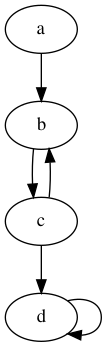
\includegraphics[scale=0.5]{my-diagram.png}
  \caption{Sample State Diagram}
  \label{fig:state-diagram}
\end{figure}

Figure \ref{fig:state-diagram} shows a state diagram.

\section{Conclusion}
\kant[42][1-3]
\end{document}
